% ŠABLONA PRO PSANÍ ZÁVĚREČNÉ STUDIJNÍ PRÁCE
%%%%%%%%%%%%%%%%%%%%%%%%%%%%%%%%%%%%%%%%%%%%
% Autor: Jakub Dokulil (kubadokulil99@gmail.com)
% Tato šablona byla vytvořena tak, aby pomocí ní mohli v systému LaTeX soutěžící sázet své práce a zároveň odpovídala požadavkům na formátování vyplývajícím z wordové šablony umístěné na webu soc.cz.
%
\documentclass[12pt, a4paper,
oneside,      %% -- odkomentujte, pokud chcete svou práci mít pouze jednostrannou, mezera pro hřbet pak automaticky bude pouze na levé straně
%twoside,        %% -- pro oboustranné práce, mezera pro hřbet následně střídá strany.
openright
]{report}

%% Nutné balíčky a nastavení
%%%%%%%%%%%%%%%%%%%%%%%%%%%%

%% Proměnné
\newcommand\obor{INFORMAČNÍ TECHNOLOGIE} %% -- napiš číslo a název tvého oboru
\newcommand\kodOboru{18-20-M/01} %% -- napiš číslo a název tvého oboru
\newcommand\zamereni{se zaměřením na počítačové sítě a programování} %% -- napiš číslo a název tvého oboru
\newcommand\skola{Střední škola průmyslová a umělecká, Opava} %% vyplň název školy
\newcommand\trida{IT4} %% vyplň jméno svého konzultanta
\newcommand\jmenoAutora{Ondřej Vícha}  %% vyplň své jméno
\newcommand\skolniRok{2023/24} %% vyplň rok
\newcommand\datumOdevzdani{1. 1. 2024} %% vyplň rok
\newcommand\nazevPrace{Webová aplikace pro zobrazení 3D modelů} %% vyplň název své práce

\title{\nazevPrace} %% -- Název tvé práce
\author{\jmenoAutora} %% -- tvé jméno
\date{\datumOdevzdani} %% -- rok, kdy píšeš SOČku

\usepackage[top=2.5cm, bottom=2.5cm, left=2.5cm, right=2.5cm]{geometry} %% nastaví okraje, left -- vnitřní okraj, right -- vnější okraj

\usepackage[czech]{babel} %% balík babel pro sazbu v češtině
\usepackage[utf8]{inputenc} %% balíky pro kódování textu
\usepackage[T1]{fontenc}
\usepackage{cmap} %% balíček zajišťující, že vytvořené PDF bude prohledávatelné a kopírovatelné

\usepackage{graphicx} %% balík pro vkládání obrázků

\usepackage{subcaption} %% balíček pro vkládání podobrázků

\usepackage{hyperref} %% balíček, který v PDF vytváří odkazy

\linespread{1.25} %% řádkování
\setlength{\parskip}{0.5em} %% odsazení mezi odstavci


\usepackage[pagestyles]{titlesec} %% balíček pro úpravu stylu kapitol a sekcí
\titleformat{\chapter}[block]{\scshape\bfseries\LARGE}{\thechapter}{10pt}{\vspace{0pt}}[\vspace{-22pt}]
\titleformat{\section}[block]{\scshape\bfseries\Large}{\thesection}{10pt}{\vspace{0pt}}
\titleformat{\subsection}[block]{\bfseries\large}{\thesubsection}{10pt}{\vspace{0pt}}


\usepackage{tocloft} % Balíček umožní přizpůsobit vzhled tabulky obsahu
\setlength{\cftbeforechapskip}{0pt}  % Menší rozestup pro kapitoly
\setlength{\cftbeforesecskip}{0pt}   % Menší rozestup pro sekce

\setcounter{secnumdepth}{2}
\setcounter{tocdepth}{2}

\usepackage{fancyhdr}
\pagestyle{fancy}
\fancyhf{}
\renewcommand{\headrulewidth}{0pt}
\fancyfoot[c]{\thepage}


\usepackage{booktabs}

\usepackage{url}

%% Balíčky co se můžou hodit :) 
%%%%%%%%%%%%%%%%%%%%%%%%%%%%%%%

\usepackage{pdfpages} %% Balíček umožňující vkládat stránky z PDF souborů, 

\usepackage{upgreek} %% Balíček pro sazbu stojatých řeckých písmen, třeba u jednotky mikrometr. Například stojaté mí: \upmu, stojaté pí: \uppi

\usepackage{amsmath}    %% Balíčky amsmath a amsfonts 
\usepackage{amsfonts}   %% pro sazbu matematických symbolů
\usepackage{esint}     %% pro sazbu různých integrálů (např \oiint)
\usepackage{mathrsfs}
\usepackage{helvet} % Helvet font
\usepackage{mathptmx} % Times New Roman
\usepackage{Oswald} % Oswald font


%% makra pro sazbu matematiky
\newcommand{\dif}{\mathrm{d}} %% makro pro sazbu diferenciálu, místo toho
%% abych musel psát '\mathrm{d}' mi stačí napsat '\dif' což je mnohem 
%% kratší a mohu si tak usnadnit práci

\usepackage{listings}
\usepackage{xcolor}


\renewcommand{\lstlistingname}{Kód}% Listing -> Algorithm
\renewcommand{\lstlistlistingname}{Seznam programových kódů}% List of Listings -> List of Algorithms

%% Definice 
\lstdefinelanguage{JavaScript}{
	morekeywords=[1]{break, continue, delete, else, for, function, if, in,
		new, return, this, typeof, var, void, while, with},
	% Literals, primitive types, and reference types.
	morekeywords=[2]{false, null, true, boolean, number, undefined,
		Array, Boolean, Date, Math, Number, String, Object},
	% Built-ins.
	morekeywords=[3]{eval, parseInt, parseFloat, escape, unescape},
	sensitive,
	morecomment=[s]{/*}{*/},
	morecomment=[l]//,
	morecomment=[s]{/**}{*/}, % JavaDoc style comments
	morestring=[b]',
	morestring=[b]"
}[keywords, comments, strings]


\lstdefinelanguage[ECMAScript2015]{JavaScript}[]{JavaScript}{
	morekeywords=[1]{await, async, case, catch, class, const, default, do,
		enum, export, extends, finally, from, implements, import, instanceof,
		let, static, super, switch, throw, try},
	morestring=[b]` % Interpolation strings.
}

\lstalias[]{ES6}[ECMAScript2015]{JavaScript}

% Nastavení barev
% Requires package: color.
\definecolor{mediumgray}{rgb}{0.3, 0.4, 0.4}
\definecolor{mediumblue}{rgb}{0.0, 0.0, 0.8}
\definecolor{forestgreen}{rgb}{0.13, 0.55, 0.13}
\definecolor{darkviolet}{rgb}{0.58, 0.0, 0.83}
\definecolor{royalblue}{rgb}{0.25, 0.41, 0.88}
\definecolor{crimson}{rgb}{0.86, 0.8, 0.24}

% Nastavení pro Python
\lstdefinestyle{Python}{
	language=Python,
	backgroundcolor=\color{white},
	basicstyle=\ttfamily,
	breakatwhitespace=false,
	breaklines=false,
	captionpos=b,
	columns=fullflexible,
	commentstyle=\color{mediumgray}\upshape,
	emph={},
	emphstyle=\color{crimson},
	extendedchars=true,  % requires inputenc
	fontadjust=true,
	frame=single,
	identifierstyle=\color{black},
	keepspaces=true,
	keywordstyle=\color{mediumblue},
	keywordstyle={[2]\color{darkviolet}},
	keywordstyle={[3]\color{royalblue}},
	literate=%
	{á}{{\'a}}1 {č}{{\v{c}}}1 {ď}{{\v{d}}}1 {é}{{\'e}}1 {ě}{{\v{e}}}1
	{í}{{\'i}}1 {ň}{{\v{n}}}1 {ó}{{\'o}}1 {ř}{{\v{r}}}1 {š}{{\v{s}}}1
	{ť}{{\v{t}}}1 {ú}{{\'u}}1 {ů}{{\r{u}}}1 {ý}{{\'y}}1 {ž}{{\v{z}}}1,		
	numbers=left,
	numbersep=5pt,
	numberstyle=\tiny\color{black},
	rulecolor=\color{black},
	showlines=true,
	showspaces=false,
	showstringspaces=false,
	showtabs=false,
	stringstyle=\color{forestgreen},
	tabsize=2,
	title=\lstname,
	upquote=true  % requires textcomp	
}


\lstdefinestyle{JSES6Base}{
	backgroundcolor=\color{white},
	basicstyle=\ttfamily,
	breakatwhitespace=false,
	breaklines=false,
	captionpos=b,
	columns=fullflexible,
	commentstyle=\color{mediumgray}\upshape,
	emph={},
	emphstyle=\color{crimson},
	extendedchars=true,  % requires inputenc
	fontadjust=true,
	frame=single,
	identifierstyle=\color{black},
	keepspaces=true,
	keywordstyle=\color{mediumblue},
	keywordstyle={[2]\color{darkviolet}},
	keywordstyle={[3]\color{royalblue}},
 literate=%
{á}{{\'a}}1 {č}{{\v{c}}}1 {ď}{{\v{d}}}1 {é}{{\'e}}1 {ě}{{\v{e}}}1
{í}{{\'i}}1 {ň}{{\v{n}}}1 {ó}{{\'o}}1 {ř}{{\v{r}}}1 {š}{{\v{s}}}1
{ť}{{\v{t}}}1 {ú}{{\'u}}1 {ů}{{\r{u}}}1 {ý}{{\'y}}1 {ž}{{\v{z}}}1,		
	numbers=left,
	numbersep=5pt,
	numberstyle=\tiny\color{black},
	rulecolor=\color{black},
	showlines=true,
	showspaces=false,
	showstringspaces=false,
	showtabs=false,
	stringstyle=\color{forestgreen},
	tabsize=2,
	title=\lstname,
	upquote=true  % requires textcomp
}

\lstdefinestyle{JavaScript}{
	language=JavaScript,
	style=JSES6Base,
}
\lstdefinestyle{ES6}{
	language=ES6,
	style=JSES6Base
}


%% Bordel pro práci - můžeš smáznout :) 
%%%%%%%%%%%%%%%%%%%

\usepackage{lipsum} %% balíček který píše lipsum (nesmyslný text, který se používá pro kontrolu typografie)
\usepackage{dirtree}
\usepackage{enumitem}
%% Začátek dokumentu
%%%%%%%%%%%%%%%%%%%%
\begin{document}
	
	\pagestyle{empty}
	\pagenumbering{Roman}
	
	\cleardoublepage

%% Titulní stránka s informacemi
%%%%%%%%%%%%%%%%%%%%%%%%%%%%%%%%%%%%%%%%
	
	{\fontfamily{phv}\selectfont
		%% Logo školy
		\begin{figure}[h]
			\centering
			
\includegraphics[width=0.6\linewidth]{image/logo-skoly.png} 
		\end{figure}
		
		
		%% Hlavička práce a její název (viz proměnná \nazev prace)
		%% \sffamily %%% bezpatkové písmo - sans serif
		{\bfseries %%% písmo na stránce je tučně
			\begin{center}
				\vspace{0.025 \textheight}
				\LARGE{ZÁVĚREČNÁ STUDIJNÍ PRÁCE}\\
				\large{dokumentace}\\
				\vspace{0.075 \textheight}
				\LARGE {\nazevPrace}\\
			\end{center}  
		}%%%
		
		\begin{figure}[h]
			\centering
			
\includegraphics[width=0.2\linewidth]{image/logo-background.png} 
		\end{figure}
		
		\vspace{0.02 \textheight}
		\begin{table}[h!]
			\begin{tabular}{ll}
				\textbf{Autor:} & \jmenoAutora\\ 
				\textbf{Obor:} & \kodOboru { } \obor\\
				\textbf{} & \zamereni\\
				\textbf{Třída:} & \trida\\
				\textbf{Školní rok:} & \skolniRok\\
			\end{tabular}
			
		\end{table}		
	}
	
\newpage %% Zalomení dvojstránky
	
%% Stránka obsahující poděkování a prohlášení
%%%%%%%%%%%%%%%%%%%%%%%%%%%%%%%%%%%%%%%%%%%%%%%%%%%%%%%%

%% Poděkování - nepovinné
%%%%%%%%%%%%%%%%%%%%%%%%%%%%
	\clearpage
	\noindent{\large{\bfseries{Poděkování}\\}}
	\noindent Chtěl bych poděkovat panu učiteli Mgr. Markovi Lučnému za užitečné rady při tvorbě projektu.
	
	\vspace*{0.7\textheight} %% Vertikální mezeru je možné upravit

%% Prohlášení - povinné
%%%%%%%%%%%%%%%%%%%%%%%%%%%%
	\noindent{\large{\bfseries{Prohlášení}\\}}  %% uprav si koncovky podle toho na jaký rod se cítíš, vypadá to pak lépe :) 
	\noindent{Prohlašuji, že jsem závěrečnou práci vypracoval samostatně a uvedl veškeré použité 
		informační zdroje.\\}
	\noindent{Souhlasím, aby tato studijní práce byla použita k výukovým a prezentačním účelům na Střední průmyslové a umělecké škole v Opavě, Praskova 399/8.}
	\vfill
	\noindent{V Opavě \datumOdevzdani\\}
	\noindent
	\begin{minipage}{\linewidth}
		\hspace{9.5cm} 
		\begin{tabular}{@{}p{6cm}@{}}
			\dotfill \\
			Podpis autora
		\end{tabular}
	\end{minipage}
	
	

%% Stránka obsahující abstrakt (anotaci)
%%%%%%%%%%%%%%%%%%%%%%%%%%%%%%%%%%%%%%%%%%%%%%%%%%%%%%%%	

%% Abstrakt v češtině
%%%%%%%%%%%%%%%%%%%%%%%%%%%%
	\noindent{\Large{\bfseries{Abstrakt}\\}}
	\noindent Tento projekt je zaměřen na vytvoření webové aplikace umožňující snadné zobrazení a stahování 3D modelů. Základem pro tento projekt je databáze MySQL a framework Django, který nabízí různé vestavěné šablony. Databáze MySQL slouží jako úložiště pro 3D modely a další související informace. Cílem je vytvořit webovou aplikaci, která nejen vizuálně působí atraktivně, ale také je snadno ovladatelná pro uživatele, kteří chtějí zobrazovat a stahovat 3D modely. \\
	\vspace{18pt}
	
	\noindent{\large{\bfseries{Klíčová slova}}}
	
	\noindent Django, MySQL, 3D, webová stránka, modely, databáze.. \dots 
	
	\vspace{18pt}
	
	\cleardoublepage %% Zalomení stránky
% předefinování příkazu chapter
\let\oldchapter\chapter
\renewcommand{\chapter}{
    \clearpage %Zajišťuje že nová kapitola začne na nové stránce
    \pagestyle{fancy} %Nastavuje styl stránky, který chcete používat
    \oldchapter
}
	\tableofcontents
%% Stránka s generovaným obsahem
%%%%%%%%%%%%%%%%%%%%%%%%%%%%%%%%%%%%%%%	
	
	%% Vygeneruje tabulku s obsahem

	\pagenumbering{arabic} %% Nastavení způsobu číslování stránek (alternativy roman | Roman)
	\setcounter{page}{4} %% Nastavení počitadla stránek

%% Stránka s úvodem - povinná část
%%%%%%%%%%%%%%%%%%%%%%%%%%%%%%%%%%%%%%%		
	\chapter*{Úvod}
%Tento příkaz vytvoří novou kapitolu s názvem "Úvod" ve vašem dokumentu.
%Hvězdička * u příkazu \chapter* znamená, že tato kapitola nebude mít číslo. Ve výsledném dokumentu se tedy objeví jako "Úvod" bez předcházejícího čísla kapitoly, které se obvykle zobrazuje u číslovaných kapitol.
%Tento příkaz také znamená, že kapitola se automaticky neobjeví v obsahu, protože LaTeX standardně zahrnuje do obsahu pouze číslované kapitoly.
	
	\addcontentsline{toc}{chapter}{Úvod}
%Tento příkaz ručně přidává záznam do obsahu.
%První parametr toc označuje, že přidáváme záznam do Table of Contents (obsahu).
%Druhý parametr chapter specifikuje úroveň záznamu. V tomto případě říkáme, že přidávaný záznam má být považován za kapitolu.
%Třetí parametr Úvod je text, který se objeví v obsahu. V tomto případě bude v obsahu zobrazen název "Úvod".	
Cílem bylo sestavení webové aplikace se zobrazením a stáhnutím 3D modelů co nejpřehledněji. Aplikace by měla obsahovat registraci a přihlášení uživatelů  pro nahrání 3D modelů i s možností hodnocení modelů a zobrazení jiných uživatelů. Uživatel by měl mít možnost upravit si vlastní profil o různé informace a taky přidat nebo upravit různé informace o vlastních modelech. Všechny model jsou přehledně na jedné stránce kde je možnost filtrace modelů. Celá webová stránka by měla být responzivní, aby fungovala na jiných zařízeních.

Nepřihlášený uživatel bude mít možnost pouze registrace, přihlášení nebo zobrazení a stáhnutí modelů zatímco přihlášený uživatel bude moct kromě těchto funkčností také hodnotit modely ostatních a také nahrávat a upravovat své vlastní modely.

V rámci projektové dokumentace se zaměřuji na postup tvorby konkrétní aplikace. Začínám analýzou databázového modelu v úvodní části. Následně se věnuji správě uživatelských účtů, implementaci formulářů pro přidání a editaci dat a vytváření pohledů pro prezentaci modelů a uživatelů. V závěrečné části se pak soustředím na design samostatné vizuální stránky a její přizpůsobení pro různá zařízení.

%Tipy k psaní úvodu
%Je povinný, nadpis neměňte, rozsah - max. 1 strana. 
%Tato část práce obsahuje: 
%* náhled do řešené problematiky, zdůvodnění volby problematiky, 
%* předem definované cíle práce, 
%* motivaci pro další čtení textu včetně stručného uvedení obsahu následujících kapitol 

\let\cleardoublepage\clearpage

\chapter{Teoretické a metodické základy}

\section{Záměr}
\label{sec:uvod}

Webové aplikace pro zobrazení 3D modelů poskytují prostor pro interaktivní prezentaci třírozměrných objektů přes internet. Tyto aplikace mohou být využívány v různých odvětvích, včetně designu, vzdělávání, průmyslu, umění a mnoha dalších. Existuje několik webových aplikací, ve kterých je možné si zobrazit 3D modely, ale většina z nich je placená a složitá. To jsou některé z důvodů, proč jsem si vybral právě tento projekt.

\section{Architektura databázových aplikací}
\label{sec:architektura}
Framework Django nabízí 2 architektury. Architektura MVC a MVT. V tomto projektu využívám architekturu MVT protože v případě MVC musí programátoři napsat veškerý kód specifický pro ovládací prvky, zatímco v případě MVT se o část týkající se kontroléru stará samotný framework. 
\begin{figure}[h]
			\centering
			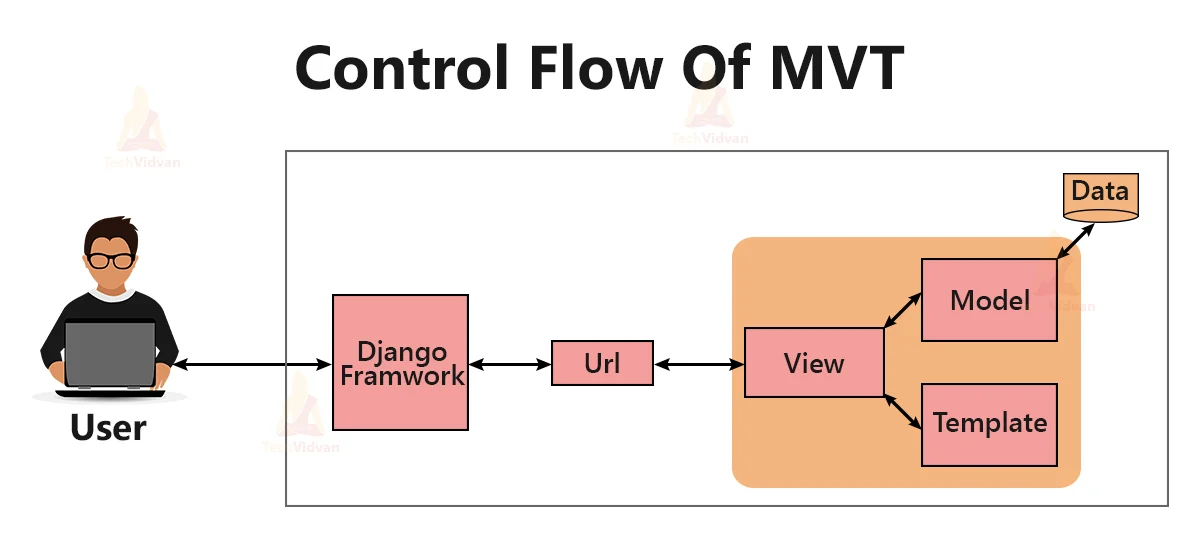
\includegraphics[width=1\linewidth]{image/mvt.png} 
			\caption{Logika MVT}
			\label{fig:mvc}
\end{figure}
\newpage
Model bude sloužit jako rozhraní pro vaše data. Je zodpovědný za údržbu dat. Je to logická struktura dat, která stojí za celou aplikací, a je reprezentována databází (zpravidla relační databází, jako je MySql, Postgres).

Zobrazení je uživatelské rozhraní - to, co vidíte v prohlížeči při vykreslování webové stránky. Je reprezentováno soubory HTML/CSS/Javascript.

Šablona se skládá ze statických částí požadovaného výstupu HTML a také z určité speciální syntaxe popisující, jak bude vložen dynamický obsah.
\section[Počáteční zkušenosti]{Počáteční zkušenosti}
Během třetího ročníku jsem se věnoval tvorbě databázových aplikací v rámci frameworku Django a manipulaci obsahu v databázi MySQL. Zaměřil jsem se na využití generických funkcí a implementaci uživatelského systému v souladu s nativními možnostmi, které Django poskytuje. Cílem bylo vytvořit funkční aplikaci s minimálním úpravami standardních prvků frameworku. Pro správu databáze jsem preferoval nástroj phpMyAdmin, který mi umožnil snadné provádění operací nad databází přes webové rozhraní. Tyto dovednosti vytvořily pevný základ pro mé další projekty v oblasti databázového vývoje.
\section[Využité technologie]{Využité technologie}
	\subsection[Django]{Django} 
	Django je svobodný a open-source webový framework napsaný v programovacím jazyce Python. Byl vyvinut pro podporu rychlého a efektivního vývoje webových aplikací. Django poskytuje komplexní sadu nástrojů a funkcí, které usnadňují vývoj webových projektů.
	\subsection[MySQL]{MySQL}  
	MySQL je open-source relační databázový systém, který poskytuje efektivní a spolehlivé ukládání a správu dat. Jedná se o jeden z nejpopulárnějších databázových systémů, a to zejména ve světě webového vývoje. MySQL podporuje mnoho jazyků programování, a je běžně používán pro ukládání dat webových aplikací, obchodních systémů, a dalších typů softwaru.
	\newpage
	\subsection[Bootstrap 4.4.1]{Bootstrap 4.4.1} 
	Bootstrap je open-source framework pro vývoj responsivních a mobilně přizpůsobivých webových stránek. Bootstrap poskytuje sadu nástrojů, stylů a komponent, které zjednodušují a urychlují proces vývoje webových aplikací. Bootstrap je napsán v jazyce HTML, CSS a JavaScript. Verze Bootstrap 4.4.1 je konkrétní verze tohoto frameworku. Každá verze Bootstrap obsahuje aktualizace, opravy chyb a nové funkce oproti předchozím verzím.
	\subsection[Aframe.js]{Aframe.js}
	A-Frame je open-source framework pro vytváření a vývoj virtuální reality (VR) a 3D scén na webu. Je postaven na jazyce JavaScript a běží v prohlížeči, což umožňuje vytvářet interaktivní a prostorové zážitky přímo ve webovém prostředí. A-Frame bylo vyvinuto společností Mozilla a je distribuováno pod licencí MIT.
A-Frame je vhodný pro tvorbu různých typů projektů, včetně virtuálních prohlídek, interaktivních edukativních aplikací, her a dalších 3D prostorových zážitků na webu.
	\chapter{Použité postupy při práci}
	\section[Založení projektu]{Založení projektu}
	Celý projekt byl vytvářen v PyCharmu. Prvním krokem bylo založení Django projektu, který původně obsahoval vestavěnou databázi SQLite. Po pečlivém zvážení jsem se rozhodl změnit databázi na MySQL z důvodů zabezpečení a rozšířené funkcionality. Následně jsem v projektu vytvořil vlastní aplikaci a měl jsem tak základní kostru stránky. Poté jsem se mohl pustit do vytváření modelů.
	\section[Databázový model]{Databázový model}
		\begin{figure}[h]
			\centering
			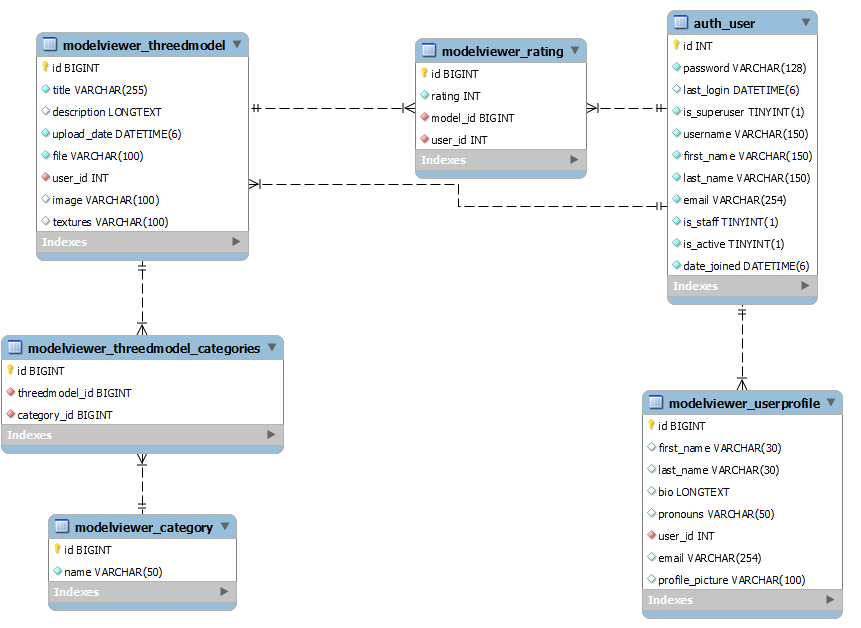
\includegraphics[width=0.9\linewidth]{image/mvt-model.png} 
			\caption{ER diagram mé webové aplikace vytvořený pomocí MySQL Workbench}
		\end{figure}
		\clearpage
		\subsection[Vztah modelu s kategoriemi]{Vztah modelu s kategoriemi} Nejdůležitější je tabulka na nahrání a popis 3D modelů u kterého si i ve vztahu N:1 můžeme vybrat více kategorií pro jeden model díky tabulce která obsahuje cizí klíče a tím funguje jako spojovací tabulka mezi nahráním 3D modelu a přidáním kategorií.
		\subsection[Vztah uživatele s profilem]{Vztah uživatele s profilem}
		Součástí diagramu je také tabulka uživatele která zajišťuje registraci, přihlášení a pravomoc uživatele. Vztah N:1 zajišťuje aby uživatelé měli jen jeden profil který můžou libovolně upravovat.
		\subsection[Vztah modelu a uživatele]{Vztah modelu a uživatele}
		Jeden model může být propojen s více hodnocením ale každé hodnocení může být propojeno pouze s jedním modelem. Modely můžou být propojeny s jedním uživatelem, ale každý uživatel může být propojen pouze s jedním modelem. Jeden uživatel může mít mnoho hodnocení, ale každé hodnocení patří pouze jednomu uživateli. 
	\newpage	
	\section[Autentizace a autorizace]{Autentizace a autorizace}
	
Uživatelský systém, který řídí přihlašování a registraci uživatelů, je klíčovým prvkem každé aplikace. Je nezbytné zajistit, aby uživatelé měli přístup pouze k těm akcím, které neporušují integritu a chod aplikace. Pro řešení této problematiky jsem se rozhodl využít vestavěný model uživatele v rámci frameworku Django, konkrétně balíčku django-contrib-auth-models. Tento balíček poskytuje robustní implementaci uživatelského modelu nazvaného User, který slouží k reprezentaci uživatelů v systému.
		
		\begin{figure}[h]
			\centering
			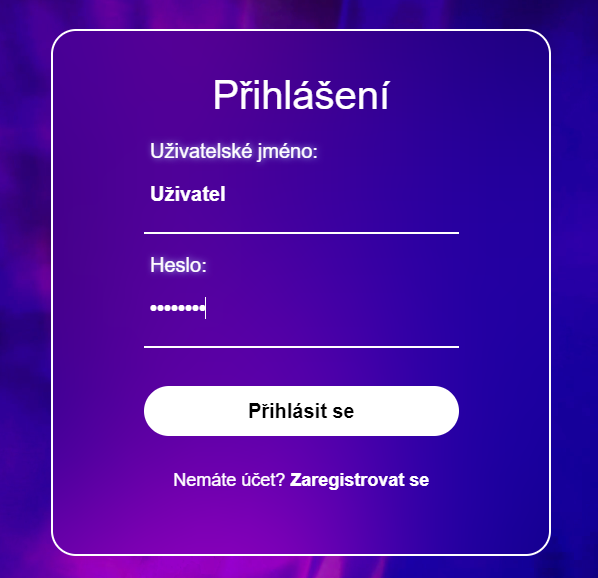
\includegraphics[width=0.518\linewidth]{image/login.png} 
			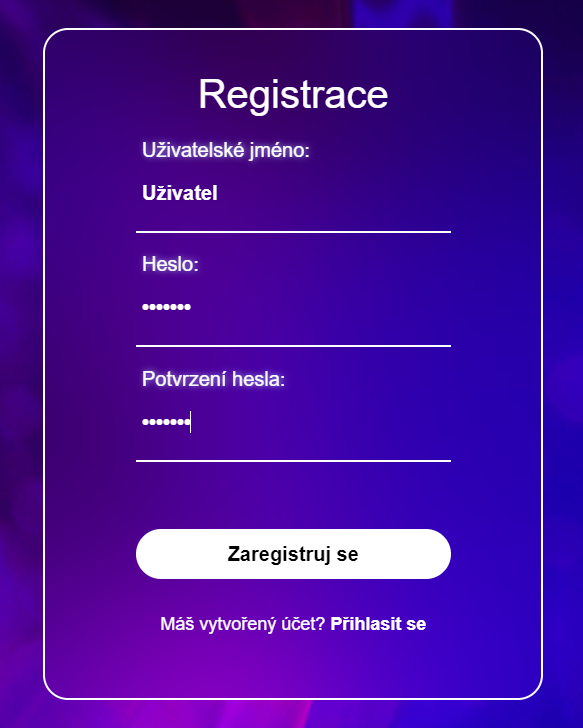
\includegraphics[width=0.4\linewidth]{image/register.png} 
			\caption{Formulář na přihlášení a registraci}
		\end{figure}
Při využití modelu User z balíčku django-contrib-auth-models získávám celou řadu funkcionalit, která usnadňuje správu uživatelů. Tento model obsahuje atributy a metody, které umožňují bezpečné ukládání hesel, ověřování přihlašovacích údajů a mnoho dalšího. Díky této integraci mohu snadno implementovat přihlašování a registraci s minimálním úsilím a s důrazem na bezpečnostní standardy.
		
Jedním z klíčových prvků je řízení přístupových práv uživatelů. Django-contrib-auth-models nabízí robustní systém oprávnění, který umožňuje definovat, ke kterým částem aplikace může uživatel přistupovat a jaké akce může provádět. To zajišťuje, že uživatelé mají pouze oprávnění nezbytná pro správný chod aplikace a minimalizuje riziko možných neoprávněných činností.
		
		\clearpage	
	\section[Operace s uživatelským účtem]{Operace s uživatelským účtem}
Uživateli jsou umožněny základní operace s jejich účtem.	
\begin{itemize}[label=\(\bullet\)]
  \item Přidání osobních informací
  \item Přidání profilového obrázku který se zobrazí v seznamu uživatelů
  \item Přidání emailu
  \item Změna hesla
\end{itemize}	
Aby k těmto funkcím měl uživatel snadný přístup, vytvořil jsem v navigační liště bloky, které se zobrazí pouze pokud je uživatel přihlášený a odkazují na podstránky řešící dané funkce.
\subsection[Úprava profilu]{Úprava profilu}
\begin{figure}[h]
			\centering
			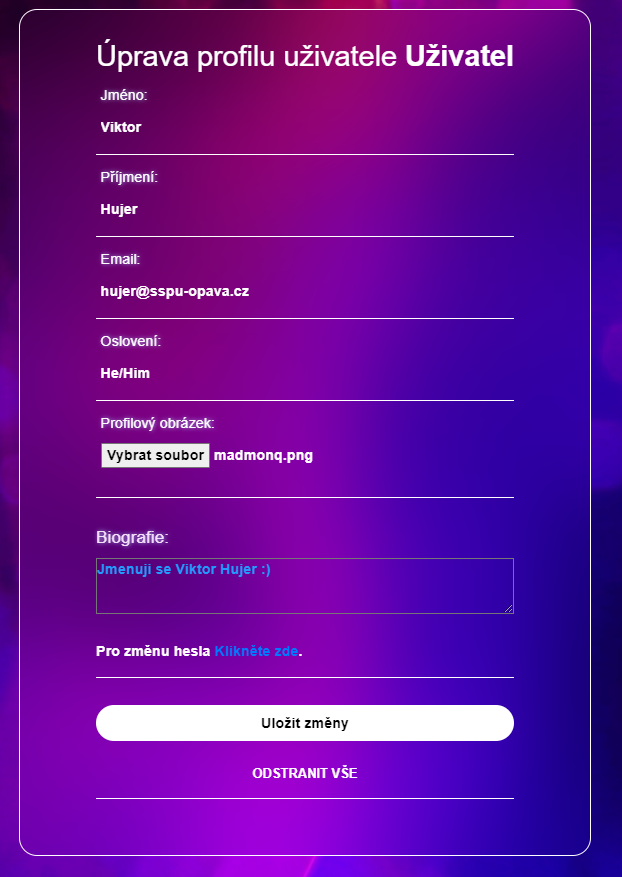
\includegraphics[width=0.5\linewidth]{image/profile.png} 
			\caption{Formulář úpravu profilu}
		\end{figure}
		
Tento formulář slouží k shromažďování klíčových informací o uživateli, zahrnující jeho osobní údaje, jako jsou jméno, příjmení, e-mailová adresa, preferovaná oblast zaměření, profilový obrázek a stručná biografie. Formulář není pouze prostředkem pro shromažďování informací, ale také představuje možnost zlepšení uživatelské interakce a začlenění jednotlivců do naší platformy. Kromě toho obsahuje praktickou možnost změny hesla, což přispívá k bezpečnosti účtu uživatele. Odkaz na další formulář pro změnu hesla umožňuje uživatelům snadno a bezpečně aktualizovat své přihlašovací údaje podle svých potřeb a preferencí.
\subsection[Změna hesla]{Změna hesla}
Uživatel by měl mít jednoduchý a snadný přístup k formuláři. Toto by mělo být realizováno prostřednictvím jasně označeného odkazu nebo tlačítka ve vhodné části uživatelského rozhraní.

\begin{figure}[h]
			\centering
			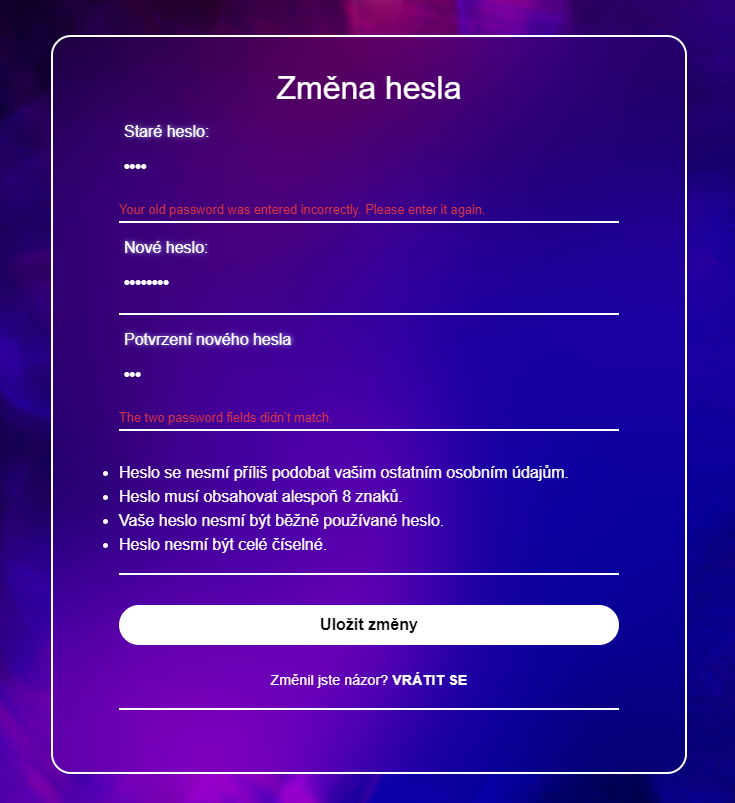
\includegraphics[width=0.5\linewidth]{image/change-password.png} 
			\caption{Formulář na změnu hesla}
		\end{figure}
		Formulář pro změnu hesla je klíčovým prvkem pro uživatelskou bezpečnost a pohodlí. Při jeho implementaci je důležité dbát na bezpečnostní standardy a poskytnout uživatelům jasný a intuitivní proces změny hesla.
		\newpage
	\section[Přidání modelu]{Přidání modelu}
	Uživatel bude mít možnost přidat do systému vlastní 3D model a obohatit jej o různé parametry a podrobnosti, které poskytnou uživatelům lepší představu o daném modelu. Tato možnost umožní uživatelům efektivněji procházet a vyhledávat mezi dostupnými 3D modely, protože budou schopni využít filtry a specifikovat požadované parametry při hledání.
	
	Databáze následně prezentuje tyto modely ostatním uživatelům, kteří mohou prohlížet, hodnotit a stahovat modely dle svých potřeb. Uživatelská interakce s modelem je klíčová, protože umožňuje tvůrcům získat zpětnou vazbu od komunity a vylepšit své modely na základě reálných potřeb uživatelů. Pro uživatele, kteří nahráli model, je k dispozici přehled vlastních modelů, což umožňuje snadný přístup k informacím, aktualizacím a případným budoucím úpravám. 
	
Důležitým a klíčovým prvkem v konfiguraci modelu jsou definované kategorie, které slouží k jeho zařazení do specifických typů. Tímto způsobem můžeme efektivně filtrovat a organizovat modely podle konkrétních charakteristik. V rámci této konfigurace jsou dostupné základní kategorie umožňující přesnější a cílenější třídění.


Významným parametrem je také přípona souboru s modelem, která je klíčová pro správnou integraci s Aframe. Pro optimální kompatibilitu a funkčnost je nutné, aby modely používaly přípony .glb nebo .gltf, neboť Aframe pracuje výhradně s těmito typy souborů. Tím je zajištěno plynulé a bezproblémové propojení modelu s danou platformou.

Kromě technických specifikací je důležité pamatovat i na estetický a vizuální prvek prezentace modelu. Fotografie, která slouží k prezentaci modelu, hraje klíčovou roli při zaujímání uživatelů. Tato fotografie je rovněž zobrazena v náhledu modelu pro všechny uživatele, což přispívá k atraktivitě a přehlednosti prezentovaného obsahu.

	
	\newpage	
	\subsection[Filtrace]{Filtrace}
	
	Vytvoření funkcí ve views.py poskytuje uživateli široké možnosti filtrování a řazení modelů v aplikaci. S pomocí těchto funkcí může uživatel přesně specifikovat požadovaná kritéria pro nalezení konkrétních modelů.
	\begin{figure}[h]
			\centering
			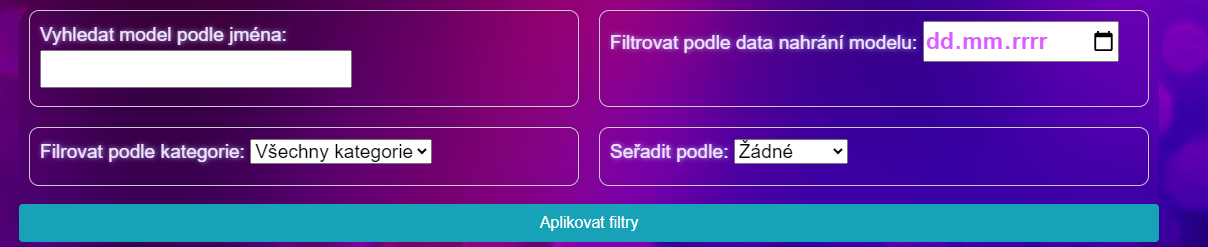
\includegraphics[width=1\linewidth]{image/Filtrace.png} 
			\caption{Filtrování}
	\end{figure}
\lstset { %
    language=Python,
    backgroundcolor=\color{black!5}, % set backgroundcolor
    basicstyle=\footnotesize,% basic font setting
}

\begin{lstlisting}
user_uploaded_models = ThreeDModel.objects.filter(user=request.user)
    categories = Category.objects.all()
    
    category_id = request.GET.get('category')
    upload_date = request.GET.get('upload_date')
    model_name = request.GET.get('model_name')
    sort_by = request.GET.get('sort_by')
   
    if category_id:
        user_uploaded_models = user_uploaded_models.filter(categories__id=category_id)
    
    if upload_date:
        user_uploaded_models = user_uploaded_models.filter(upload_date=upload_date)
   
    if model_name:
        user_uploaded_models = user_uploaded_models.filter(Q(title__icontains=model_name))
   
    if sort_by == 'newest':
        user_uploaded_models = user_uploaded_models.order_by('-upload_date')
    elif sort_by == 'oldest':
        user_uploaded_models = user_uploaded_models.order_by('upload_date')
    return render(request, 'user/profile.html', {'user_uploaded_models':
     user_uploaded_models,'categories': categories})
\end{lstlisting}
Tahle funkce v views.py zajistí filtraci v zobrazení vlastních modelů \dots



Filtraci lze provádět podle různých parametrů, včetně jména modelu, data nahrání a kategorií. To umožňuje uživateli rychle a efektivně najít požadované modely v rozsáhlé databázi. Díky této funkcionalitě má uživatel možnost upravit zobrazení výsledků podle svých individuálních preferencí a potřeb.

Kromě toho je uživatel schopen řadit modely podle data nahrání, a to buď od nejstarších po nejnovější, nebo naopak. Tato možnost řazení umožňuje uživateli organizovat výsledky tak, jak nejlépe odpovídá jeho požadavkům a usnadňuje rychlé porovnání modelů.

Celkově vzato, díky implementaci těchto funkcí ve views.py získává uživatel vysokou flexibilitu a přesnost při procházení a vyhledávání modelů v aplikaci. To zlepšuje uživatelskou zkušenost a umožňuje snadné a intuitivní používání aplikace pro správu a prohlížení modelů.
		
		\subsection[Editace]{Editace}
		Uživatelovi je poskytnuta možnost upravit svůj nahraný model podle vlastních představ a potřeb. K tomu slouží interaktivní formulář, který umožňuje měnit a přizpůsobovat různé části modelu podle specifických požadavků uživatele.

\begin{figure}[h]
			\centering
			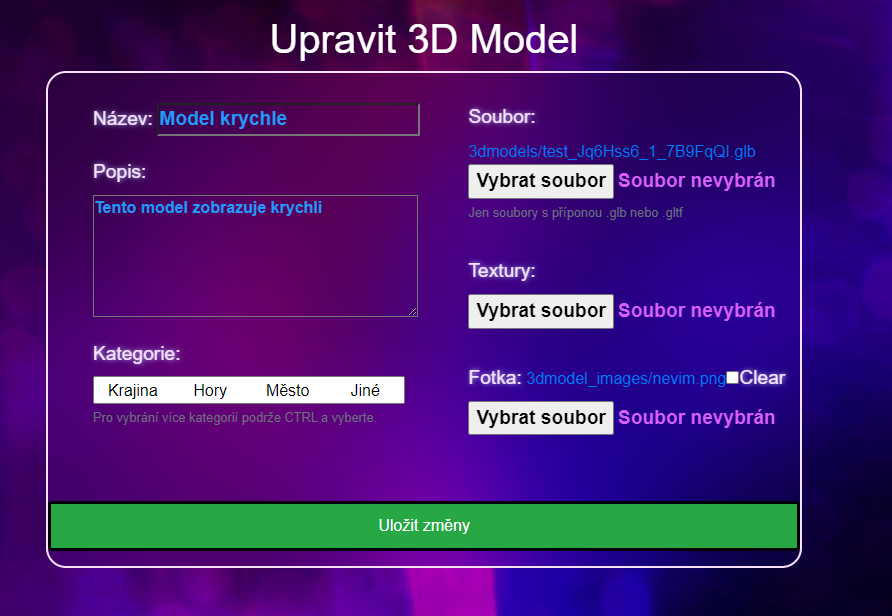
\includegraphics[width=1\linewidth]{image/edit.png} 
			\caption{Formulář editace}
		\end{figure}
		
Tento formulář zobrazuje uživateli obsah, který měl původně nahraný v různých částech modelu, takže má jasný přehled o tom, co již bylo vytvořeno. Každá část, kterou uživatel rozhodne upravit, je snadno dostupná pro editaci. Může měnit text, parametry a další klíčové prvky podle svého uvážení.


Tato interaktivní možnost úpravy umožňuje uživateli vylepšit a personalizovat svůj model, aby co nejlépe odpovídal jeho potřebám a preferencím. Tímto způsobem má uživatel plnou kontrolu nad tím, jakým směrem se vyvíjí jeho vlastní model, a může ho dále zdokonalovat podle svých aktuálních požadavků.
\subsection[Zobrazení na stránce]{Zobrazení na stránce}
Představení modelu je způsobem prezentace, který využívá karty k zobrazení klíčových informací o každém modelu. Každá karta obsahuje vizuální obrázek, název a průměrné hodnocení daného modelu, což umožňuje uživatelům rychle získat přehled o dostupných modelech. Při najetí myší na konkrétní kartu se automaticky zobrazí podrobnější informace, včetně údajů jako jméno uživatele, který model nahrál, popis samotného modelu a datum, kdy byl model nahrán do systému.

\begin{figure}[h]
			\centering
			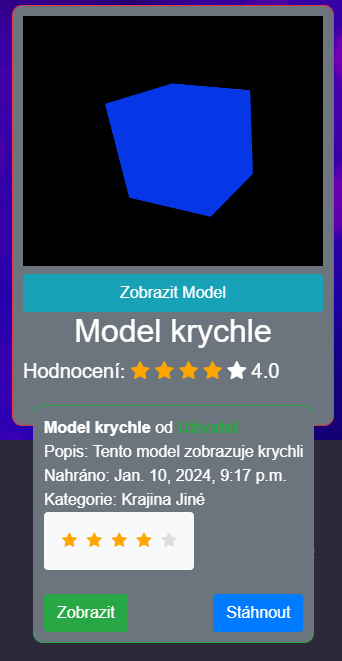
\includegraphics[width=0.3\linewidth]{image/model-view.png} 
			\caption{Zobrazení modelů}
		\end{figure}
		
Tato funkce poskytuje uživatelům příležitost získat hlubší vhled do každého modelu, a to vše na jednom uživatelském rozhraní. Kromě toho je implementována funkce, která umožňuje hodnocení modelu od 1 do 5 hvězdiček, pokud uživatel, který hodnotí, není tvůrcem daného modelu. Tato bezpečnostní opatření zajistí, že hodnocení poskytují pouze uživatelé, u nichž není střet zájmů a kteří mohou poskytnout objektivní zpětnou vazbu.
\newpage
\chapter[Zobrazení modelu]{Zobrazení modelu}
\section[Aframe]{Aframe}
Zobrazení modelů bylo implementováno pomocí A-Frame. Tato jednoduchá možnost umožňuje vytvořit zobrazení modelů pouze s použitím běžného HTML souboru, bez nutnosti instalace dalších nástrojů. Jedinou důležitou věcí je přidat do své stránky nebo aplikace skript s odkazem na knihovnu A-Frame, a poté můžeme upravovat a přidávat prvky dle vlastního uvážení.
\begin{lstlisting}
<script src="https://aframe.io/releases/1.5.0/aframe.min.js"></script>
\end{lstlisting}
\section[Scripty]{Scripty}
\subsection[Základní zobrazení]{Základní zobrazení}
Základní kód na zobrazení modelu, který zatím řeší pouze jednoduché textury i s scriptem který zmenší velikost modelu tak aby nebyl příliš veliký v zobrazení:
\begin{lstlisting}
<a-scene class="aframebox" embedded>
      <a-assets>
          <a-asset-item id="model" src="{{ model.file.url }}"></a-asset-item>
      </a-assets>
      <a-light type="ambient" position="1 1 1" intensity="1"></a-light>
      <a-entity gltf-model="#model" modify-materials 
      	max-dimensions position="0 0 0" rotation="0 0 0"/>
      <a-camera id="camera" position="5 1.5 5" rotation="0 0 0" wasd-controls>
      	<a-cursor></a-cursor>
      </a-camera>
      <script>          </script>
</a-scene>
                  
\end{lstlisting}
Tenhle kód zajistí pozici, kameru a základní funkci zobrazení konkrétního modelu, další funkce kterými chceme zlepšit interaktivitu modelu píšeme do <script>   <script>\dots
\newpage
\subsection[Script pro zmenšení]{Script pro zmenšení}
Hlavním účelem tohoto scriptu je omezení maximálních rozměrů 3D modelu aby nebyl příliš veliký a tím pádem se lépe a rychleji zobrazil, a to automaticky při načítání scény.
\begin{lstlisting}
AFRAME.registerComponent('max-dimensions', {
   	 init: function () {
        	var maxDimensions = { x: 1, y: 1, z: 1 };
        	this.el.addEventListener('model-loaded', function () {
        		var modelDimensions = this.getObject3D
        		('model').geometry.boundingBox.getSize();
        		var scaleFactor = Math.min(
        			maxDimensions.x / modelDimensions.x,
        			maxDimensions.y / modelDimensions.y,
       				maxDimensions.z / modelDimensions.z
        		);
        		this.setAttribute('scale', scaleFactor
        		 + ' ' + scaleFactor + ' ' + scaleFactor);
        	});
   	  }
  });
\end{lstlisting}
Další scripty které můj projekt má je otáčení okolo modelu pohybem do stran nebo nahoru a dolů pomocí klávesnice, nebo také obnovení kamery na původní bod.
\subsection[Vizualizace]{Vizualizace}

\begin{figure}[h]
			\centering
			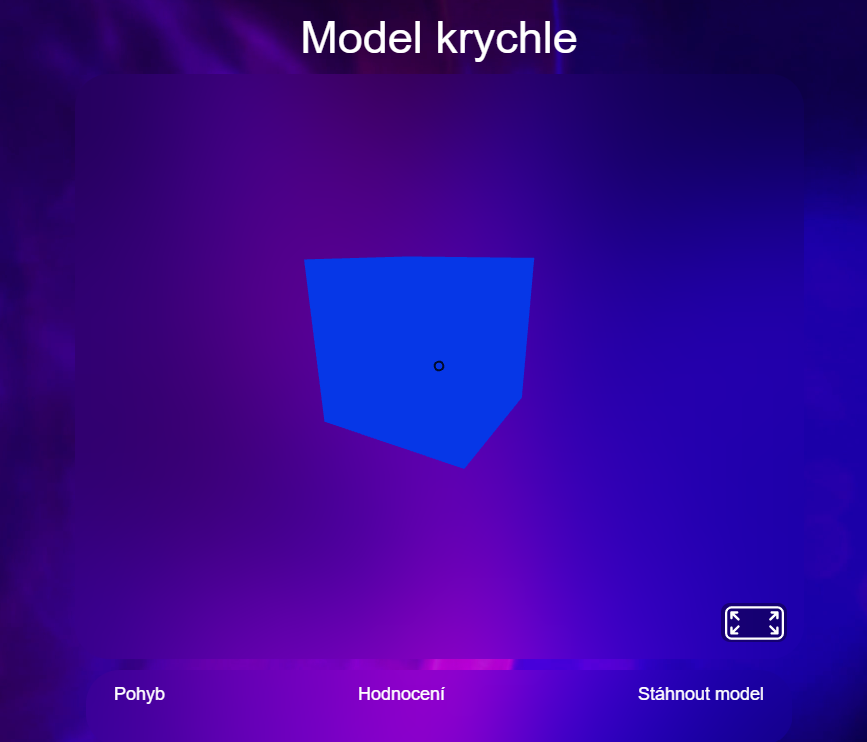
\includegraphics[width=0.5\linewidth]{image/model.png} 
			\caption{Zobrazení modelů}
		\end{figure}
		Na stránce konkrétního modelu je návod jak se dá v modelu pohybovat s kamerou pomocí klávesnice, nalezneme tam také možnost hodnocení modelu a možnost stáhnout si model.
\chapter{Výsledky řešení}
\section[Splněné a nesplněné cíle]{Splněné a nesplněné cíle}
Cíle projektu:
\begin{itemize}[label=\(\bullet\)]
  \item Vytvoření funkční webové aplikace s podporou importu a exportu 3D modelů.
  \item  Navrhnout a vytvořit základní design stránky pro přehledné zobrazení 3D modelů.
  \item Získat relevantní informace a poznatky pro úspěšnou implementaci importu a exportu 3D modelů
  \item  Vylepšit design webové stránky pro lepší uživatelský zážitek.
   \item   Implementovat funkční přihlašování pro uživatele.
    \item   Zajištění importu modelů včetně jejich textur.
    \item   Zdockerovat webovou aplikaci.
\end{itemize}
Cílem bylo vytvořit funkční aplikaci a při jejím vytváření a vývoji pochopit řadu principů a technologií. Během vytváření a vývoje mé aplikace jsem měl za cíl nejen dosáhnout funkčnosti, ale také pochopit a implementovat řadu principů a technologií. Ačkoliv se mi podařilo dosáhnout většiny stanovených cílů a aplikace v základu funguje, narazil jsem na výzvy při zobrazení pokročilých vlastních textur. I když aplikace dosahuje požadované funkčnosti, věřím, že existuje prostor pro vylepšení v efektivitě a čitelnosti kódu.

Cílem do budoucna je nadále rozvíjet tuto aplikaci. Mám představu o možných vylepšeních a nových funkcionalitách, které by mohly přinést přidanou hodnotu uživatelům. Plánuji pracovat na odstranění nedostatků ve zobrazení pokročilých vlastních textur a současně zdokonalovat celkový kód aplikace. Pro ty, kteří by si chtěli aplikaci vyzkoušet, je k dispozici otevřený zdrojový kód na mém GitHub repositáři.
	\chapter*{Závěr}
	
	Cílem projektu bylo vytvoření webové aplikace na zobrazení 3D modelů s uživatelskými účty. Aplikace umožňuje uživatelům vytvoření, hodnocení, nahrání a stažení modelů. Aplikace je postavená na frameworku Django. Front-end je řešen pomocí klasického Html, JavaScriptu, CSS a Bootstrap 4.4.1. Na pozadí aplikace běží databázový systém MySQL. 
	
	Podle mě jsem základní cíl projektu splnil, až na nějaké menší nedostatky. V průběhu práce jsem si zopakoval práci s Djangem, kde jsem se přiučil novým komplexnějším věcem, a databází MySQL. Dále jsem porozuměl, aspoň na úrovni abych to mohl v praxi využít, frameworku Aframe.js přes který zobrazuji 3D modely. Do budoucna bych chtěl aplikaci určitě zDockerovat a také přidat hezčí design a responzivnost celé aplikace. Taky bych chtěl aplikaci zbavit pár drobných chyb které dělají horší uživatelský zážitek.
	
	Aplikace je zálohovaná na GitHub adrese https://github.com/OndraVicha/zaverecny-projekt.
	\renewcommand{\bibname}{Seznam použitých informačních zdrojů}
	%% literatura
	\begin{thebibliography}{99}
		\bibitem{Django}Django: The web framework for perfectionists with deadlines.[online]. [cit. 2023-12-30]. Dostupné z: \url{https://www.djangoproject.com/}
		\bibitem{MySQL}MySQL:  The world's most popular open source database.[online]. [cit. 2023-12-30]. Dostupné z: \url{https://www.mysql.com/}
		\bibitem{Bootstrap}Bootstrap: The most popular HTML, CSS, and JS library in the world.[online]. [cit. 2023-12-30]. Dostupné z: \url{https://getbootstrap.com/}
		\bibitem{Aframe}Aframe: A web framework for building virtual reality experiences.[online]. [cit. 2023-12-30]. Dostupné z:  \url{https://aframe.io/}
		\bibitem{sspuLogo} \textit{Střední škola průmyslová a umělecká Opava}[online]. [cit. 2023-12-30]. Dostupné z:  \url{https://www.sspu-opava.cz}
		\bibitem{MVT}MVT: Model-View-Template  [online]. [cit. 2023-12-30]. Dostupné z: \url{https://www.javatpoint.com/django-mvtm}
		\bibitem{W3Schools}W3Schools: Online Web Tutorials [online]. [cit. 2023-12-30]. Dostupné z: \url{https://www.w3schools.com/}
		\bibitem{User}User authentication in Django [online]. [cit. 2023-12-30]. Dostupné z: \url{https://docs.djangoproject.com/en/5.0/topics/auth/}
		\bibitem{MySQLWorkBench}MySQLWorkBench: a unified visual tool for database architects, developers, and DBAs [online]. [cit. 2023-12-30]. Dostupné z: \url{https://www.mysql.com/products/workbench/}

	\end{thebibliography}
	\newpage
	%% obrázky 
	\listoffigures
	
	
	
	\appendix %% začínají přílohy
	
	\titleformat{\chapter}[block]{\scshape\bfseries\LARGE}{Příloha \thechapter}{10pt}{\vspace{0pt}}[\vspace{-22pt}] %% nastavení nadpisu u příloh
	
	
	
	
\end{document}